\documentclass[11pt,a4paper]{article}
\usepackage[margin=2cm]{geometry}
\usepackage{graphicx}
\usepackage{xcolor}
\usepackage{tcolorbox}
\usepackage{enumitem}
\usepackage{multicol}
\usepackage{amsmath}
\usepackage{amssymb}
\usepackage{fancyhdr}
\usepackage{hyperref}
\usepackage{tikz}
\usetikzlibrary{arrows.meta, positioning, shapes, patterns}

% Define colors
\definecolor{mlblue}{RGB}{31, 119, 180}
\definecolor{mlorange}{RGB}{255, 127, 14}
\definecolor{mlgreen}{RGB}{44, 160, 44}
\definecolor{mlred}{RGB}{214, 39, 40}
\definecolor{mlpurple}{RGB}{148, 103, 189}

% Header and footer
\pagestyle{fancy}
\fancyhf{}
\lhead{Week 1: Innovation Exercises}
\rhead{Clustering for Innovation}
\cfoot{Page \thepage}

\title{\Large\textbf{Innovation Through Clustering:\\Practical Discovery Exercises}\\
\vspace{0.5em}
\large Take-Home Innovation Challenges - Week 1}
\author{BSc Machine Learning for Innovation\\
\textit{Individual or Team Exercises}}
\date{}

\begin{document}
\maketitle
\thispagestyle{fancy}

\begin{tcolorbox}[colback=mlgreen!10, colframe=mlgreen!50, title={\textbf{Exercise Objective}}]
Apply clustering concepts to real innovation challenges. Each exercise builds from simple observation to strategic implementation. Complete at least 3 exercises for full understanding.
\end{tcolorbox}

\section*{Exercise 1: Customer Feedback Clustering}

\subsection*{Scenario}
You're working with a food delivery startup that has 100 customer complaints from last month. They need to identify the main problem areas to prioritize fixes.

\subsection*{Data Sample (First 10 complaints):}
\begin{enumerate}[label=\arabic*.]
\item ``Food was cold when it arrived''
\item ``Driver couldn't find my address''
\item ``App crashed during payment''
\item ``Food took 90 minutes to arrive''
\item ``Missing items from my order''
\item ``Payment was charged twice''
\item ``Driver was rude''
\item ``Food quality was poor''
\item ``App wouldn't accept my coupon''
\item ``Delivery time estimate was wrong''
\end{enumerate}

\subsection*{Tasks:}

\textbf{A. Manual Clustering (10 min)}
\begin{itemize}
\item Group similar complaints together
\item Name each cluster (e.g., ``Delivery Issues'')
\item Count complaints per cluster
\end{itemize}

\begin{tcolorbox}[colback=white, colframe=gray!50]
\textbf{Your Clusters:}
\begin{enumerate}
\item Cluster Name: \underline{\hspace{6cm}} Count: \underline{\hspace{1cm}}
\item Cluster Name: \underline{\hspace{6cm}} Count: \underline{\hspace{1cm}}
\item Cluster Name: \underline{\hspace{6cm}} Count: \underline{\hspace{1cm}}
\item Cluster Name: \underline{\hspace{6cm}} Count: \underline{\hspace{1cm}}
\end{enumerate}
\end{tcolorbox}

\textbf{B. Innovation Opportunities (10 min)}

For each cluster, propose one innovation:

\begin{center}
\begin{tabular}{|p{4cm}|p{8cm}|}
\hline
\textbf{Problem Cluster} & \textbf{Innovation Solution} \\
\hline
& \\[1cm]
\hline
& \\[1cm]
\hline
& \\[1cm]
\hline
& \\[1cm]
\hline
\end{tabular}
\end{center}

\textbf{C. Priority Matrix (5 min)}

Plot your solutions on Impact vs Effort:

\begin{center}
\begin{tikzpicture}[scale=0.6]
\draw[->] (0,0) -- (10,0) node[right] {Implementation Effort};
\draw[->] (0,0) -- (0,10) node[above] {Customer Impact};
\draw[gray!30] (0,5) -- (10,5);
\draw[gray!30] (5,0) -- (5,10);
\node at (2.5,7.5) {\small Quick Wins};
\node at (7.5,7.5) {\small Strategic};
\node at (2.5,2.5) {\small Low Priority};
\node at (7.5,2.5) {\small Consider Later};
\end{tikzpicture}
\end{center}

\newpage
\section*{Exercise 2: Product Feature Space}

\subsection*{Scenario}
Your team has brainstormed 15 features for a new fitness app. You need to group them into coherent releases.

\subsection*{Features with Attributes:}
\begin{center}
\small
\begin{tabular}{|l|c|c|c|}
\hline
\textbf{Feature} & \textbf{Dev Time (weeks)} & \textbf{User Value (1-10)} & \textbf{Technical Risk (1-10)} \\
\hline
Social sharing & 2 & 7 & 3 \\
AI coach & 8 & 9 & 9 \\
Progress graphs & 1 & 6 & 2 \\
Video tutorials & 3 & 8 & 4 \\
Meal planner & 4 & 7 & 5 \\
Heart rate monitor & 2 & 8 & 6 \\
Community forum & 3 & 6 & 3 \\
Workout library & 2 & 9 & 2 \\
Personal records & 1 & 7 & 2 \\
Music integration & 2 & 5 & 4 \\
Virtual races & 5 & 6 & 7 \\
Habit tracker & 2 & 8 & 3 \\
Coach messaging & 4 & 7 & 6 \\
Calorie counter & 2 & 8 & 3 \\
Equipment finder & 3 & 4 & 5 \\
\hline
\end{tabular}
\end{center}

\subsection*{Tasks:}

\textbf{A. 3D Clustering Challenge}

Using the three dimensions (Dev Time, User Value, Risk), identify natural groupings:

\begin{tcolorbox}[colback=white, colframe=mlblue!50]
\textbf{Group 1: ``\underline{\hspace{6cm}}''}\\
Features: \underline{\hspace{10cm}}\\[0.5cm]
\textbf{Group 2: ``\underline{\hspace{6cm}}''}\\
Features: \underline{\hspace{10cm}}\\[0.5cm]
\textbf{Group 3: ``\underline{\hspace{6cm}}''}\\
Features: \underline{\hspace{10cm}}
\end{tcolorbox}

\textbf{B. Release Planning}

Based on your clusters, create a 3-release roadmap:

\begin{center}
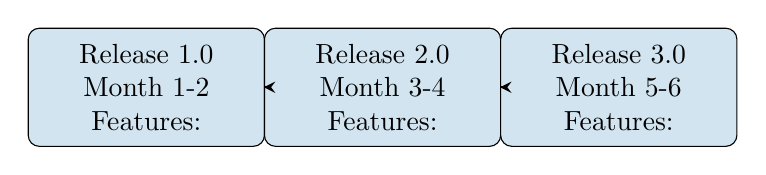
\begin{tikzpicture}[node distance=3cm]
\tikzstyle{release} = [rectangle, rounded corners, minimum width=3cm, minimum height=1.5cm, text centered, draw=black, fill=mlblue!20]
\tikzstyle{arrow} = [thick,->,>=stealth]

\node (r1) [release, align=center] {Release 1.0\\Month 1-2\\Features:};
\node (r2) [release, right of=r1, align=center] {Release 2.0\\Month 3-4\\Features:};
\node (r3) [release, right of=r2, align=center] {Release 3.0\\Month 5-6\\Features:};

\draw [arrow] (r1) -- (r2);
\draw [arrow] (r2) -- (r3);
\end{tikzpicture}
\end{center}

\newpage
\section*{Exercise 3: Innovation Ecosystem Mapping}

\subsection*{Scenario}
Map your organization's innovation initiatives to find gaps and overlaps.

\subsection*{Innovation Dimensions:}

\begin{center}
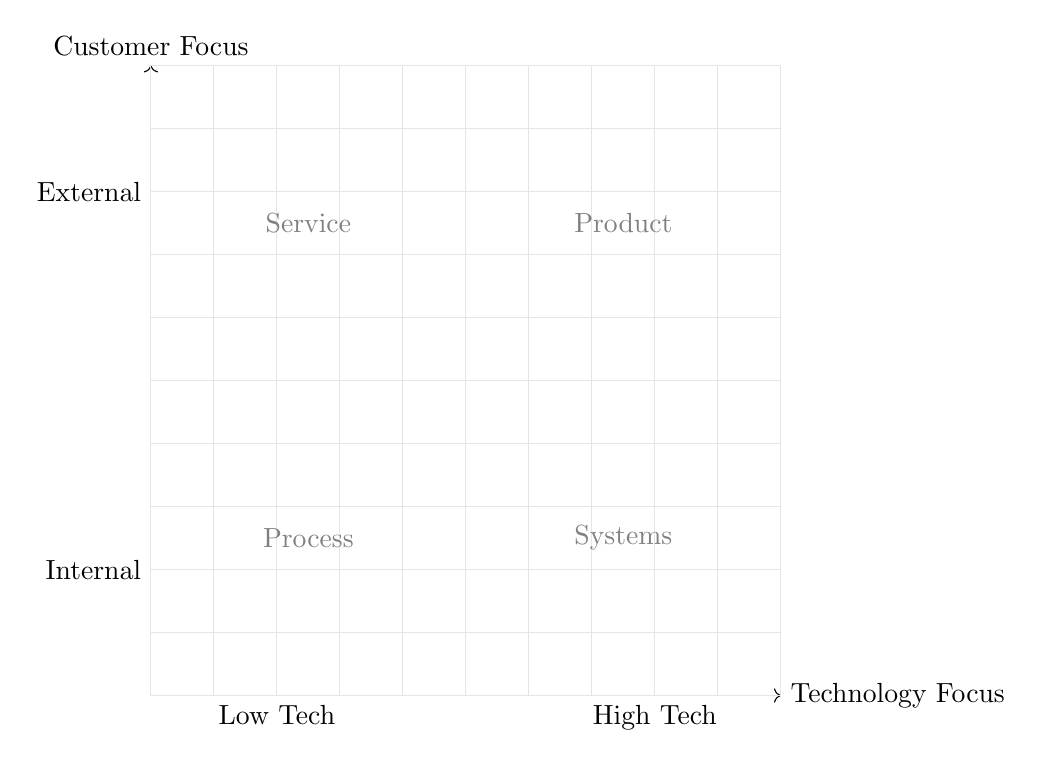
\begin{tikzpicture}[scale=0.8]
% Axes
\draw[->] (0,0) -- (10,0) node[right] {Technology Focus};
\draw[->] (0,0) -- (0,10) node[above] {Customer Focus};

% Labels
\node[below] at (2,0) {Low Tech};
\node[below] at (8,0) {High Tech};
\node[left] at (0,2) {Internal};
\node[left] at (0,8) {External};

% Grid
\draw[gray!20] (0,0) grid (10,10);

% Quadrants
\node[gray] at (2.5,2.5) {Process};
\node[gray] at (7.5,2.5) {Systems};
\node[gray] at (2.5,7.5) {Service};
\node[gray] at (7.5,7.5) {Product};
\end{tikzpicture}
\end{center}

\subsection*{Tasks:}

\textbf{A. Plot Your Initiatives}

Think of 10 current or potential innovation projects in your domain. Plot them above.

\textbf{B. Cluster Analysis}

\begin{enumerate}
\item Which quadrant has the most initiatives? \underline{\hspace{4cm}}
\item Which quadrant is empty (white space)? \underline{\hspace{4cm}}
\item Do you see any natural clusters? Describe: \underline{\hspace{6cm}}
\end{enumerate}

\textbf{C. Strategic Insights}

\begin{tcolorbox}[colback=mlorange!10, colframe=mlorange!50]
\textbf{Gap Analysis:} What innovation opportunity exists in the white space?\\
\vspace{2cm}

\textbf{Overlap Issue:} Where are you over-investing?\\
\vspace{2cm}

\textbf{Balance Strategy:} How would you redistribute resources?\\
\vspace{2cm}
\end{tcolorbox}

\newpage
\section*{Exercise 4: Persona Discovery Through Behavior}

\subsection*{Scenario}
You have usage data from 1000 app users. Instead of demographics, you'll cluster by behavior.

\subsection*{Sample User Behaviors:}

\begin{center}
\begin{tikzpicture}[scale=0.7]
% Create scatter plot with different user types
\draw[->] (0,0) -- (10,0) node[right] {Daily Usage (minutes)};
\draw[->] (0,0) -- (0,10) node[above] {Features Used};

% Power users
\foreach \i in {1,...,8}
    \fill[mlred!70] ({7+rand*1.5},{7+rand*1.5}) circle (2pt);
    
% Regular users
\foreach \i in {1,...,15}
    \fill[mlblue!70] ({4+rand*2},{4+rand*2}) circle (2pt);
    
% Occasional users
\foreach \i in {1,...,10}
    \fill[mlgreen!70] ({1+rand*1.5},{6+rand*2}) circle (2pt);
    
% Dormant users
\foreach \i in {1,...,12}
    \fill[mlorange!70] ({0.5+rand*1},{1+rand*1}) circle (2pt);
\end{tikzpicture}
\end{center}

\subsection*{Tasks:}

\textbf{A. Behavioral Personas}

Without knowing demographics, create personas based on the usage patterns:

\begin{center}
\begin{tabular}{|l|p{4cm}|p{5cm}|}
\hline
\textbf{Persona Name} & \textbf{Behavior Pattern} & \textbf{Likely Needs} \\
\hline
``\underline{\hspace{3cm}}'' & & \\[1.5cm]
\hline
``\underline{\hspace{3cm}}'' & & \\[1.5cm]
\hline
``\underline{\hspace{3cm}}'' & & \\[1.5cm]
\hline
``\underline{\hspace{3cm}}'' & & \\[1.5cm]
\hline
\end{tabular}
\end{center}

\textbf{B. Innovation for Each Persona}

Design one feature specifically for each persona:

\begin{enumerate}
\item \textbf{Persona 1 Feature:} \underline{\hspace{8cm}}
\item \textbf{Persona 2 Feature:} \underline{\hspace{8cm}}
\item \textbf{Persona 3 Feature:} \underline{\hspace{8cm}}
\item \textbf{Persona 4 Feature:} \underline{\hspace{8cm}}
\end{enumerate}

\newpage
\section*{Exercise 5: Competitive Landscape Clustering}

\subsection*{Scenario}
Analyze competitors to find your unique innovation space.

\subsection*{Competitor Attributes Matrix:}

Create your own analysis for 5 competitors in your field:

\begin{center}
\begin{tabular}{|l|c|c|c|c|}
\hline
\textbf{Competitor} & \textbf{Price Level} & \textbf{Feature Count} & \textbf{Market Share} & \textbf{Innovation Rate} \\
& (1-10) & (1-10) & (\%) & (Updates/Year) \\
\hline
\underline{\hspace{3cm}} & & & & \\[0.5cm]
\hline
\underline{\hspace{3cm}} & & & & \\[0.5cm]
\hline
\underline{\hspace{3cm}} & & & & \\[0.5cm]
\hline
\underline{\hspace{3cm}} & & & & \\[0.5cm]
\hline
\underline{\hspace{3cm}} & & & & \\[0.5cm]
\hline
\end{tabular}
\end{center}

\subsection*{Tasks:}

\textbf{A. Strategic Groups}

Based on your analysis, identify 2-3 strategic groups:

\begin{tcolorbox}[colback=white, colframe=mlpurple!50]
\textbf{Group 1:} \underline{\hspace{10cm}}\\
Members: \underline{\hspace{10cm}}\\
Strategy: \underline{\hspace{10cm}}\\[0.5cm]

\textbf{Group 2:} \underline{\hspace{10cm}}\\
Members: \underline{\hspace{10cm}}\\
Strategy: \underline{\hspace{10cm}}\\[0.5cm]

\textbf{Group 3:} \underline{\hspace{10cm}}\\
Members: \underline{\hspace{10cm}}\\
Strategy: \underline{\hspace{10cm}}
\end{tcolorbox}

\textbf{B. Blue Ocean Discovery}

Where is the uncontested market space (no cluster)?

\begin{center}
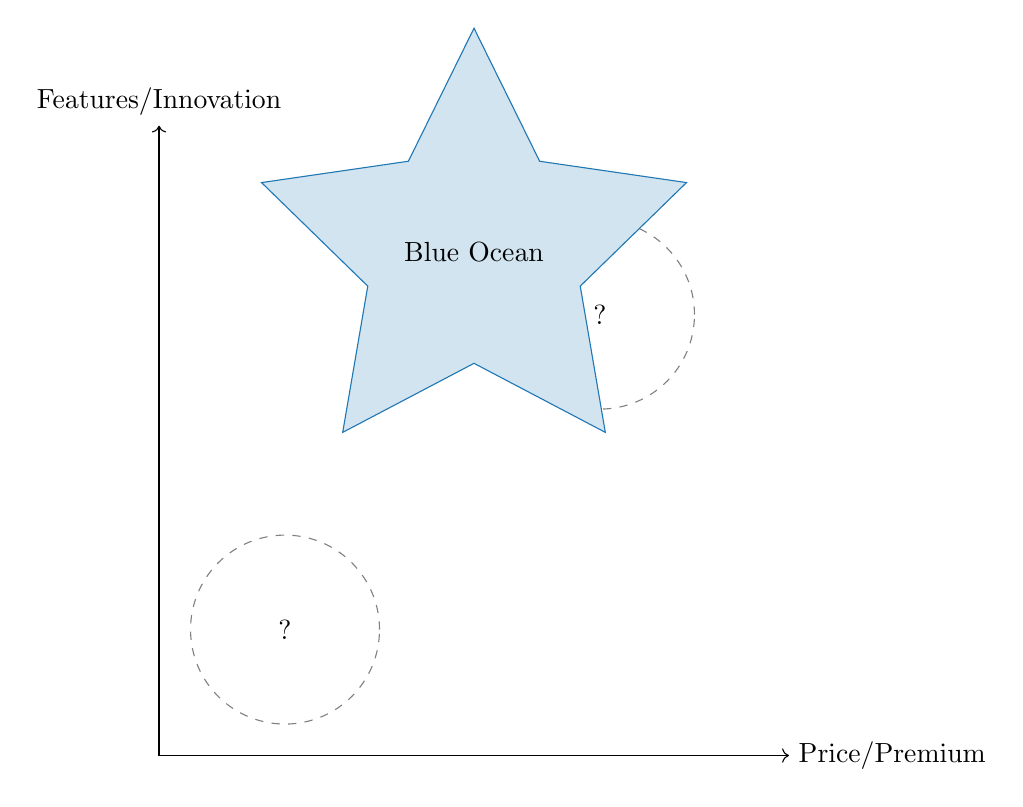
\begin{tikzpicture}[scale=0.8]
\draw[->] (0,0) -- (10,0) node[right] {Price/Premium};
\draw[->] (0,0) -- (0,10) node[above] {Features/Innovation};

% Draw your competitive clusters
\draw[dashed, gray] (2,2) circle (1.5cm);
\node at (2,2) {?};

\draw[dashed, gray] (7,7) circle (1.5cm);
\node at (7,7) {?};

% Mark blue ocean
\node[star, star points=5, star point ratio=2, draw=mlblue, fill=mlblue!20, minimum size=1cm] at (5,8) {Blue Ocean};
\end{tikzpicture}
\end{center}

\newpage
\section*{Challenge: Real-World Application}

\subsection*{Your Innovation Challenge}

Apply clustering to a real problem in your domain:

\textbf{1. Problem Definition}
\begin{tcolorbox}[colback=white, colframe=gray!50, height=3cm]
What innovation challenge are you solving?\\
\vspace{2.5cm}
\end{tcolorbox}

\textbf{2. Data/Dimensions}
\begin{tcolorbox}[colback=white, colframe=gray!50, height=3cm]
What are you clustering? What dimensions matter?\\
\vspace{2.5cm}
\end{tcolorbox}

\textbf{3. Clustering Approach}
\begin{tcolorbox}[colback=white, colframe=gray!50, height=3cm]
How will you group items? What's your distance metric?\\
\vspace{2.5cm}
\end{tcolorbox}

\textbf{4. Expected Clusters}
\begin{tcolorbox}[colback=white, colframe=gray!50, height=3cm]
What groups do you expect to find?\\
\vspace{2.5cm}
\end{tcolorbox}

\textbf{5. Innovation Actions}
\begin{tcolorbox}[colback=white, colframe=gray!50, height=3cm]
What will you do with the clustering results?\\
\vspace{2.5cm}
\end{tcolorbox}

\section*{Reflection}

\begin{tcolorbox}[colback=mlgreen!10, colframe=mlgreen!50, title={\textbf{Learning Synthesis}}]
\textbf{Key Insight:} What's the most valuable thing you learned about clustering for innovation?\\
\vspace{3cm}

\textbf{Application:} How will you use clustering in your next project?\\
\vspace{3cm}
\end{tcolorbox}

\end{document}